\documentclass{article}
\usepackage{fancyhdr}
\usepackage[utf8]{inputenc}
\usepackage[english]{babel}
\usepackage{tikz, multicol, graphicx, etoolbox, enumerate, setspace, relsize, mathrsfs, verbatim}
\usepackage{amsmath, amsfonts, amssymb, amsthm, epsfig, epstopdf, titling, url, array, esvect, tikz-3dplot}
\usepackage{graphicx}
\usepackage{hyperref}
\usepackage{listings}
\usepackage{xcolor}

\hypersetup{
    colorlinks=true,
    linkcolor=blue,
    filecolor=magenta,      
    urlcolor=cyan,
    pdftitle={Overleaf Example},
    pdfpagemode=FullScreen,
    }

\definecolor{codegreen}{rgb}{0,0.6,0}
\definecolor{codegray}{rgb}{0.5,0.5,0.5}
\definecolor{codepurple}{rgb}{0.58,0,0.82}
\definecolor{backcolour}{rgb}{0.95,0.95,0.92}

\usepackage{pgfplots}
\usepackage{tcolorbox}
\usepackage{amsthm}
\usepackage{cancel}
\usepackage[left=1in,right=1in,top=1in,bottom=1in]{geometry}
\usepackage[tableaux]{prooftrees}

\lstdefinestyle{mystyle}{
    backgroundcolor=\color{backcolour},   
    commentstyle=\color{codegreen},
    keywordstyle=\color{magenta},
    numberstyle=\tiny\color{codegray},
    stringstyle=\color{codepurple},
    basicstyle=\ttfamily\footnotesize,
    breakatwhitespace=false,         
    breaklines=true,                 
    captionpos=b,                    
    keepspaces=true,                 
    numbers=left,                    
    numbersep=5pt,                  
    showspaces=false,                
    showstringspaces=false,
    showtabs=false,                  
    tabsize=2
}

\lstset{style=mystyle}

\pagestyle{fancy}
\fancyhf{}
\fancyhead[L,RO]{Tasksheet 9}
\fancyhead[R,RO]{Fundamentals of Computational Mathematics}
\fancyfoot[L,RO]{Xiang Gao}
\fancyfoot[R,RO]{Math 4610}
\renewcommand{\headrulewidth}{0.4pt}% Default \headrulewidth is 0.4pt
\renewcommand{\footrulewidth}{0.4pt}% Default \footrulewidth is 0pt
\def\checkmark{\tikz\fill[scale=0.4](0,.35) -- (.25,0) -- (1,.7) -- (.25,.15) -- cycle;} 

\begin{document}

\section*{Task 1}
I have created the following five routines to compute the following linear algebra operations on vectors, they are all documented \href{https://github.com/GoByMark/math4610/blob/main/Homework_Tasks/Tasksheet_09/src/Task_1.py}{here} in the \href{https://github.com/GoByMark/math4610/blob/main/Homework_Tasks/Software_Manual/Software_Manual_toc.md}{Software Manual}.\\
\begin{enumerate}
\item[1.] Vector Addition\\
\lstinputlisting[language=Python]{VecAdd.py}
\item[2.] Vector Subtraction\\
\lstinputlisting[language=Python]{VecSub.py}
\item[3.] Scalar Multiplication for Vectors\\
\lstinputlisting[language=Python]{ScaMul.py}
\item[4.] Dot Product for Two Vectors of the Same Length\\
\lstinputlisting[language=Python]{DotPro.py}
\item[5.] Outer Product for Two Vectors of the Same Length\\
\lstinputlisting[language=Python]{OutPro.py}
\end{enumerate}
I have also created the following testing code that test each of the routines, 

\lstinputlisting[language=Python]{Task_1.py}

Which has the following output:
\begin{center}
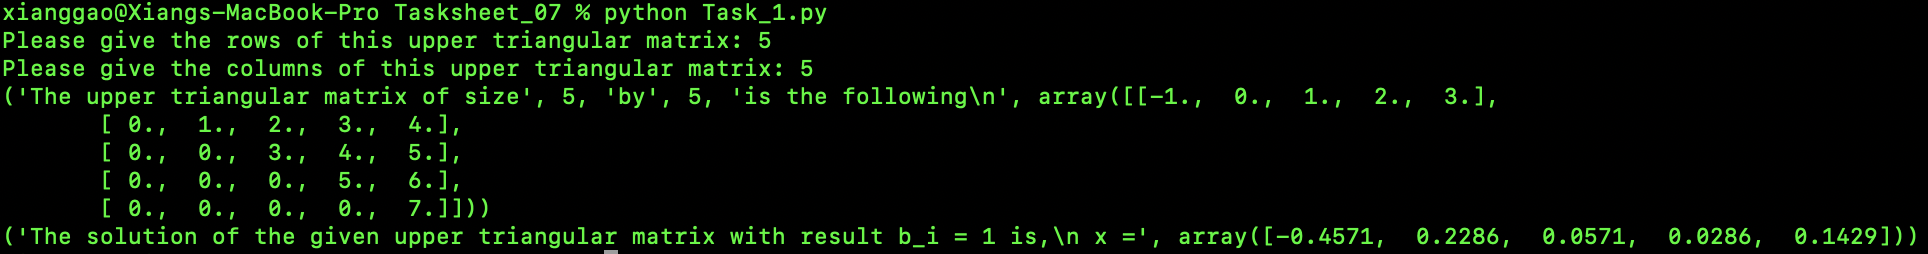
\includegraphics[width=\textwidth]{Screenshots/1.png}\\
{\bf Figure 1.} The Test Result of Each Routine from Terminal.\\

\vspace{5pt}

\includegraphics[width=\textwidth]{Screenshots/1.5.png}\\
{\bf Figure 1.5.} The Test Result of Each Routine from IDE.\\
\end{center}

\section*{Task 2}
I have created the following six routines to compute the following linear algebra operations on vectors, they are all documented \href{https://github.com/GoByMark/math4610/blob/main/Homework_Tasks/Tasksheet_09/src/Task_2.py}{here} in the \href{https://github.com/GoByMark/math4610/blob/main/Homework_Tasks/Software_Manual/Software_Manual_toc.md}{Software Manual}.\\
\begin{enumerate}
\item[1.] The magnitude of a vector - $\left(l_1\right)$ norm version\\
\lstinputlisting[language=Python]{L1_Norm.py}
\item[2.] The magnitude of a vector - $\left(l_2\right)$ norm version\\
\lstinputlisting[language=Python]{L2_Norm.py}
\item[3.] The magnitude of a vector - $\left(l_\infty\right)$ norm version\\
\lstinputlisting[language=Python]{Linf_Norm.py}
\item[4.] The error between vectors - $\left(l_1\right)$ norm version.\\
\lstinputlisting[language=Python]{L1_Norm_Error.py}
\item[5.] The error between vectors - $\left(l_2\right)$ norm version.\\
\lstinputlisting[language=Python]{L2_Norm_Error.py}
\item[6.] The error between vectors - $\left(l_\infty\right)$ norm version.\\
\lstinputlisting[language=Python]{Linf_Norm_Error.py}
\end{enumerate}
I have also created the following testing code that test each of the routines, 

\lstinputlisting[language=Python]{Task_2.py}

Which has the following output:
\begin{center}
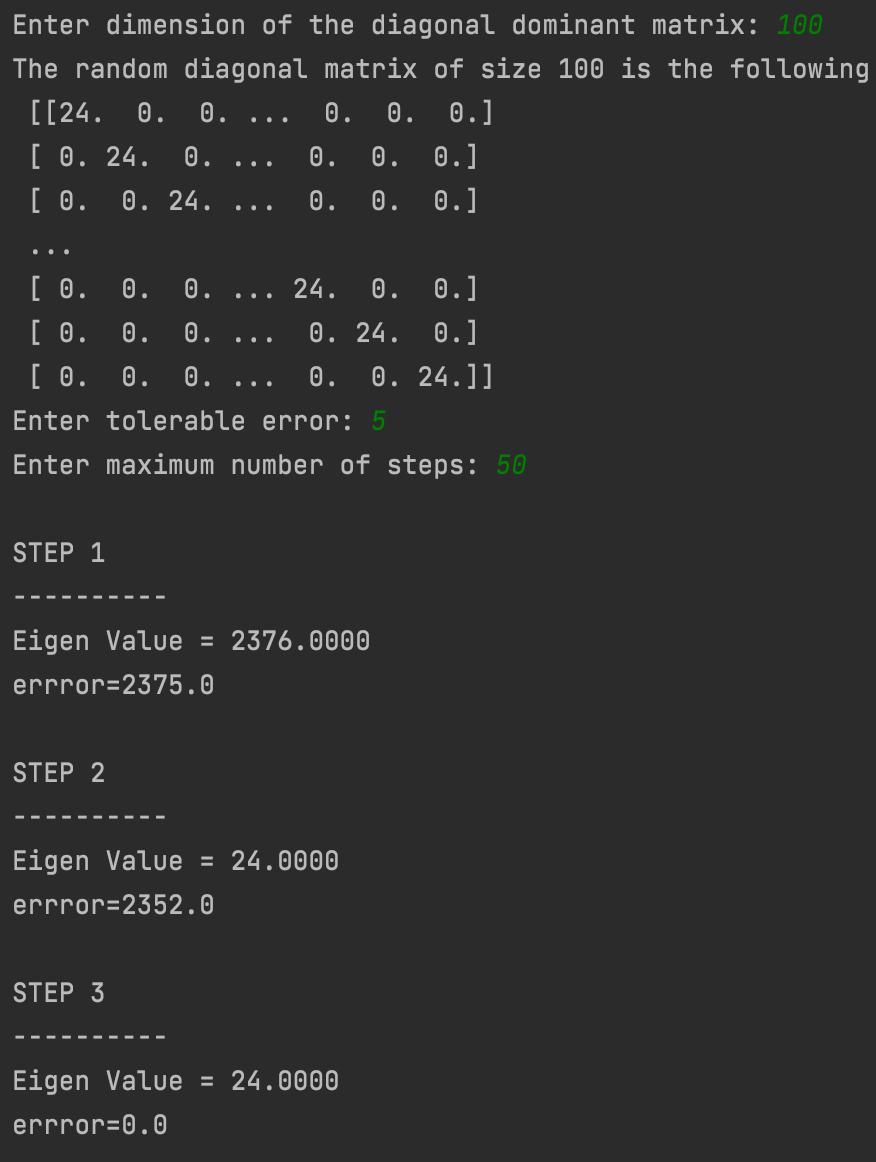
\includegraphics[width=\textwidth]{Screenshots/2.png}\\
{\bf Figure 2.} The Test Result of Each Routine from IDE.
\end{center}

\section*{Task 3}
I have created the following six routines to compute the following linear algebra operations on vectors, they are all documented \href{https://github.com/GoByMark/math4610/blob/main/Homework_Tasks/Tasksheet_09/src/Task_3.py}{here} in the \href{https://github.com/GoByMark/math4610/blob/main/Homework_Tasks/Software_Manual/Software_Manual_toc.md}{Software Manual}.\\
\begin{enumerate}
\item[1.] Matrix Addition\\
\lstinputlisting[language=Python]{matAdd.py}
\item[2.] Matrix Subtraction\\
\lstinputlisting[language=Python]{matSub.py}
\item[3.] Scalar Multiplication for a Matrix\\
\lstinputlisting[language=Python]{matScaMul.py}
\item[4.] The Transpose of a Matrix.\\
\lstinputlisting[language=Python]{matTran.py}
\item[5.] The Product of a Rectangular Matrix and Vector.\\
\lstinputlisting[language=Python]{matVecPro.py}
\item[6.] The Product of Two Rectangular Matrices.\\
\lstinputlisting[language=Python]{matMatPro.py}
\end{enumerate}
I have also created the following testing code that test each of the routines, 

\lstinputlisting[language=Python]{Task_3.py}

Which has the following output:
\begin{center}
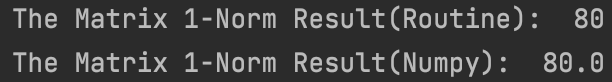
\includegraphics[width=\textwidth]{Screenshots/3.png}\\
{\bf Figure 3.} The Test Result of Each Routine from IDE.
\end{center}

\section*{Task 4}
I have written the following code to implement Jacobi Iteration for solving linear systems of equations, it's documented \href{https://github.com/GoByMark/math4610/blob/main/Homework_Tasks/Tasksheet_09/src/Task_4.py}{here} in the \href{https://github.com/GoByMark/math4610/blob/main/Homework_Tasks/Software_Manual/Software_Manual_toc.md}{Software Manual}.\\

\lstinputlisting[language=Python]{Task_4.py}

Which has the following output:
\begin{center}
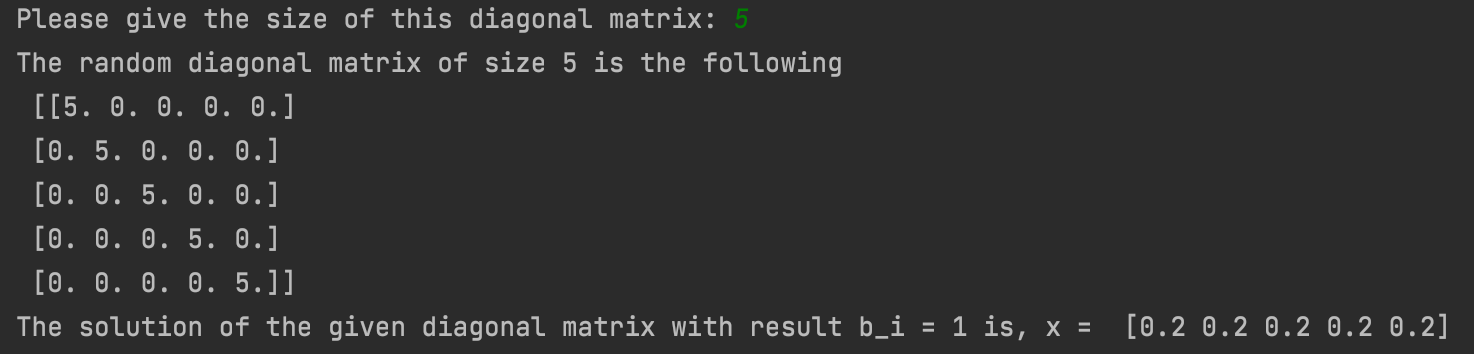
\includegraphics[width=\textwidth]{Screenshots/4.png}\\
{\bf Figure 4.} The Test Result of the Jacobi Method from Terminal.
\end{center}

\section*{Task 5}
I have written the following code to compare the results for the Gaussian elimination to the results from Jacobi Iteration for solving linear systems of equations, it's documented \href{https://github.com/GoByMark/math4610/blob/main/Homework_Tasks/Tasksheet_09/src/Task_5.py}{here} in the \href{https://github.com/GoByMark/math4610/blob/main/Homework_Tasks/Software_Manual/Software_Manual_toc.md}{Software Manual}.\\

\lstinputlisting[language=Python]{Task_5.py}

Which has the following output:
\begin{center}
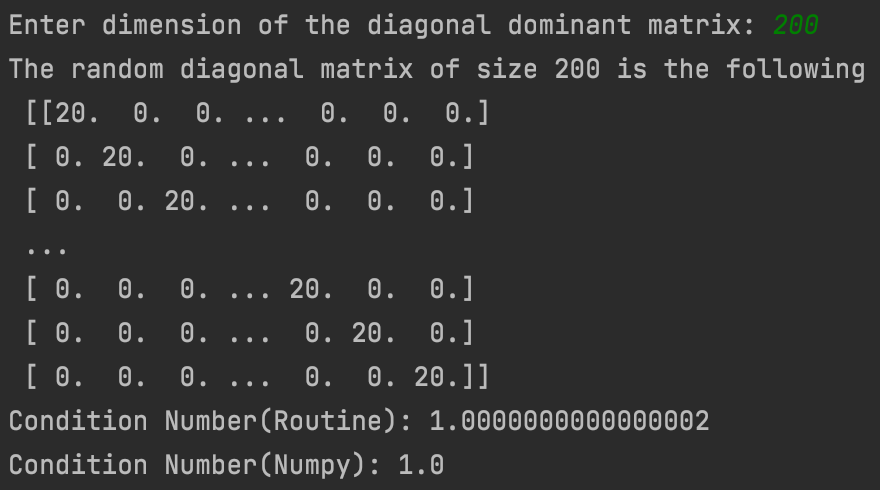
\includegraphics[width=\textwidth]{Screenshots/5.png}\\
{\bf Figure 5.} The Comparison of the Results.
\end{center}

\section*{Task 6}
In \href{https://www.math-linux.com/mathematics/linear-systems/article/gauss-seidel-method}{this website}\footnote{https://www.math-linux.com/mathematics/linear-systems/article/gauss-seidel-method} I found, the Gauss-Seidel method has a faster rate of convergence than the Jacobi Iteration. \\

The element-wise formula for the Gauss–Seidel method is extremely similar to that of the Jacobi method. However, in \href{https://johnfoster.pge.utexas.edu/numerical-methods-book/LinearAlgebra_IterativeSolvers.html}{this website}\footnote{https://johnfoster.pge.utexas.edu/numerical-methods-book/LinearAlgebra\_IterativeSolvers.html} I found,  unlike the Jacobi method, the computations for each element are generally much harder to implement in parallel, since they can have a very long critical path, and are thus most feasible for sparse matrices. Furthermore, the values at each iteration are dependent on the order of the original equations.
\end{document}